\documentclass[border=10pt]{standalone}
\usepackage{tikz}\usepackage{amsmath}
\usetikzlibrary{calc,arrows.meta}
\begin{document}
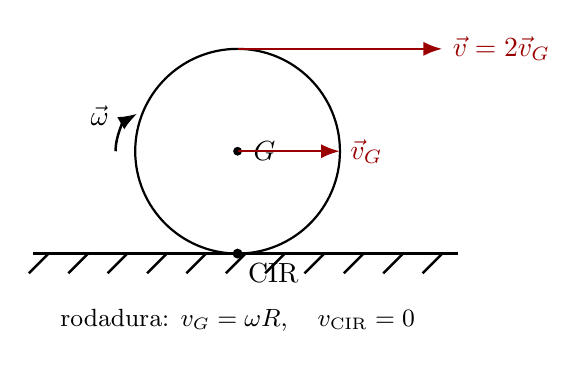
\begin{tikzpicture}[line width=0.9pt,>={Latex[length=2.4mm]}]
  % suelo
  \draw[thick] (-2.6,0)--(2.8,0);
  \foreach \x in {-2.4,-1.9,...,2.6} \draw (\x,0)--(\x-0.25,-0.25);
  % rueda
  \draw[thick] (0,1.3) circle (1.3);
  \fill (0,1.3) circle(1.6pt) node[right=2pt]{$G$};
  % CIR en el contacto
  \fill (0,0) circle(1.8pt) node[below right]{CIR};
  % velocidades
  \draw[->,red!60!black] (0,1.3)--(1.3,1.3) node[right]{$\vec v_G$};
  \draw[->,red!60!black] (0,2.6)--(2.6,2.6) node[right]{$\vec v=2\vec v_G$};
  \node at (0,0) [circle,fill=black,inner sep=1pt]{};
  % omega
  \draw[->] (-1.55,1.3) arc (180:120:0.55); \node at (-1.75,1.75){$\vec\omega$};
  % relacion
  \node at (0,-0.85){\small rodadura: $v_G=\omega R,\quad v_{\text{CIR}}=0$};
\end{tikzpicture}
\end{document}
